\documentclass[14pt]{beamer}
%
% Choose how your presentation looks.
%
% For more themes, color themes and font themes, see:
% http://deic.uab.es/~iblanes/beamer_gallery/index_by_theme.html
%
\mode<presentation>
{
  \usetheme{default}      % or try Darmstadt, Madrid, Warsaw, ...
  \usecolortheme{default} % or try albatross, beaver, crane, ...
  \usefonttheme{default}  % or try serif, structurebold, ...
  \setbeamertemplate{navigation symbols}{}
  \setbeamertemplate{caption}[numbered]
} 

\addtobeamertemplate{navigation symbols}{}{%
    \usebeamerfont{footline}%
    \usebeamercolor[fg]{footline}%
    \hspace{1em}%
    \insertframenumber/\inserttotalframenumber
}
\usepackage[english]{babel}
\usepackage[utf8x]{inputenc}
\usepackage{xcolor,colortbl}
\definecolor{Gray}{gray}{0.85}
\definecolor{LightCyan}{rgb}{0.88,1,1}

\title[Your Short Title]{Refresh Strategies for Continuous Active Learning}
\author{Nimesh Ghelani \\ Gordon V. Cormack \\ Mark D. Smucker}
\institute{University of Waterloo}
\date{First International Workshop on Professional Search, 2018}

\begin{document}
\setbeamertemplate{caption}{\raggedright\insertcaption\par}

\begin{frame}
  \titlepage
\end{frame}

% Uncomment these lines for an automatically generated outline.
%\begin{frame}{Outline}
%  \tableofcontents
%\end{frame}

% \section{Purpose}

% \begin{frame}{Purpose}
% \begin{itemize}
%     \item Discussion about my work in-progress
%     \item Get feedback and criticism
% \end{itemize}
% \end{frame}

\section{Introduction}
\begin{frame}{Introduction}
    Find all or nearly all relevant documents using minimal assessment costs
    \vskip 1cm

    \pause
    High Recall problem
    \vskip 1cm
    Some problems:
    \begin{itemize}
        \item Legal eDiscovery
        \item Systematic Review
        \item Building test collection
    \end{itemize}

\end{frame}

\begin{frame}{Introduction}
    Technology Assisted Review (TAR): computer-assisted methods to do eDiscovery

    \vskip 1cm
    \pause
    Continuous Active Learning (CAL):
    \begin{itemize}
        \item A TAR protocol
        \item Human in loop with a machine learning model
    \end{itemize}
\end{frame}

\begin{frame}{Introduction}
\begin{figure}
 \centering 
 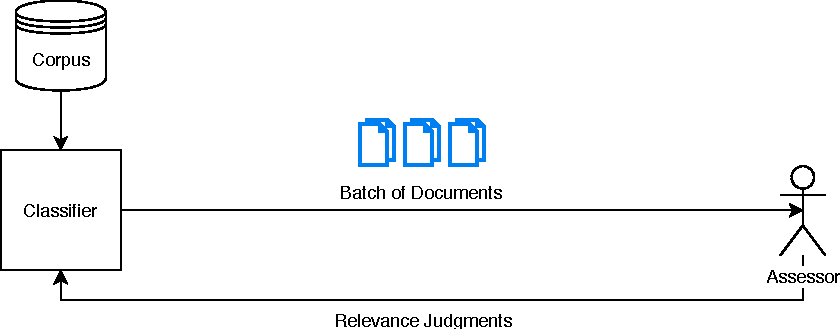
\includegraphics[width=1.0\textwidth]{animation/1.pdf}
 \caption{Relevance Feedback Loop}
\end{figure}
\end{frame}

\begin{frame}{Introduction}
\begin{figure}
 \centering 
 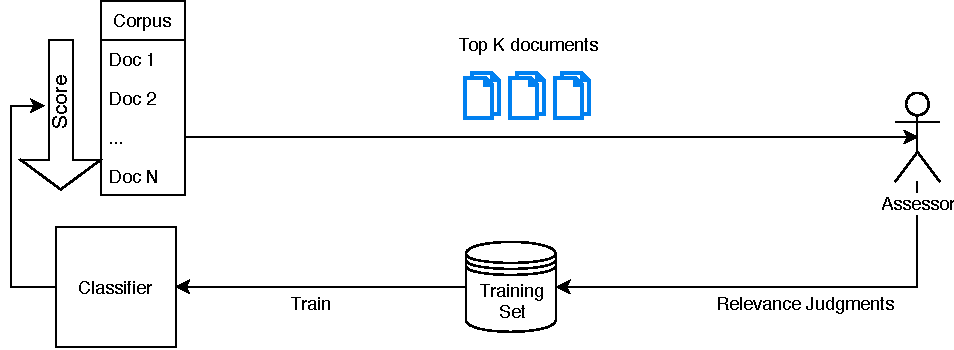
\includegraphics[width=1.0\textwidth]{animation/2.pdf}
 \caption{Relevance Feedback Loop}
\end{figure}
\end{frame}

\begin{frame}{Introduction}
\begin{figure}
 \centering 
 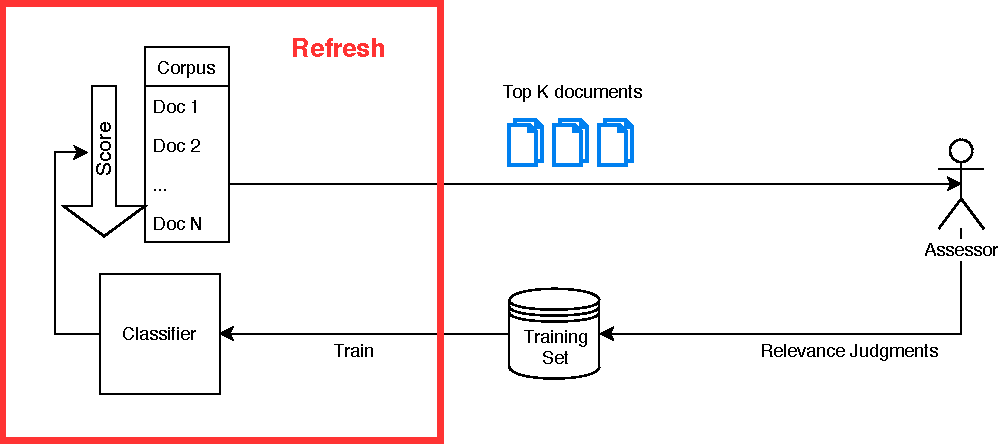
\includegraphics[width=1.0\textwidth]{animation/3.pdf}
 \caption{Relevance Feedback Loop}
\end{figure}
\end{frame}

\begin{frame}{Introduction}
Refresh:
\begin{itemize}
    \item Use available judgments to build a classifier
    \item Produce next set of documents to be judged
\end{itemize}

\pause
\vskip 1cm
Refresh Strategy
\begin{itemize}
    \item When to refresh?
    \item How to refresh?
\end{itemize}

\pause
\vskip 1cm
\textbf{Objective: }
Investigate various refresh strategies; their effectiveness and efficiency
\end{frame}

\begin{frame}{Outline}
\begin{itemize}
    \item Refresh Strategies
    \begin{itemize}
        \item Static batch sizes
        \item Partial refresh
        \item Precision based
        % \item Recency Weighting
        % \item Forgetting
    \end{itemize}
    \item Results
    \item Summary
\end{itemize}
\end{frame}

\begin{frame}{Static Batch Strategy}
\begin{figure}
 \centering 
 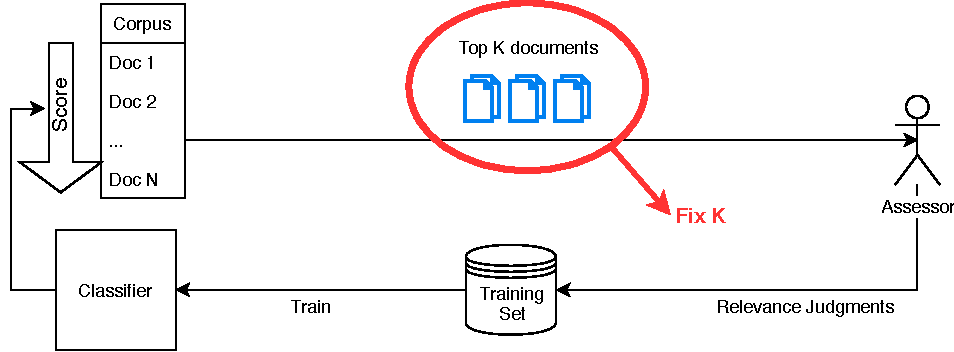
\includegraphics[width=1.0\textwidth]{animation/static.pdf}
 \caption{Static Batch Strategy}
\end{figure}
\end{frame}

\begin{frame}{BMI Strategy}
Used in the Baseline Model Implementation (BMI) at the TREC 2015 and 2016 Total
Recall tracks

\vskip 1cm
Train and score all documents every $K$ assessments ($K$ increases exponentially)

\vskip 1cm
After every refresh,
$K← K + (K + 9)/10$
\begin{figure}
\end{figure}
\end{frame}

\subsection{Partial Refresh}
\begin{frame}{Partial Refresh}
Perform frequent scoring on a smaller set of data
\vskip 0.7cm
Periodic complete scoring

% \vskip 1cm
% After every judgment:
% \begin{itemize}
%     \item train on all available judgments
%     \item re-score high ranking documents from previous full refresh
% \end{itemize}
 
% Parameters
% \begin{itemize}
%     \item Size of partial re-score document set ($s$)
%     \item Period for full refresh ($k$)
% \end{itemize}
\end{frame}


\begin{frame}{Partial Refresh Strategy}
\begin{figure}
 \centering 
 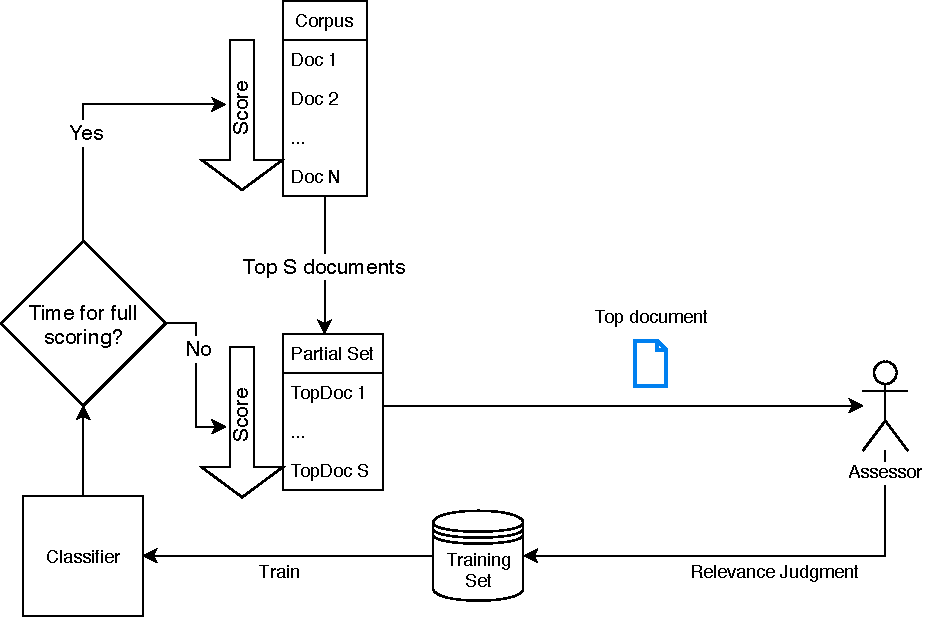
\includegraphics[width=1.0\textwidth]{animation/partial.pdf}
 \caption{Partial Refresh Strategy}
\end{figure}
\end{frame}

\begin{frame}{Partial Refresh Strategy}
\begin{figure}
 \centering 
 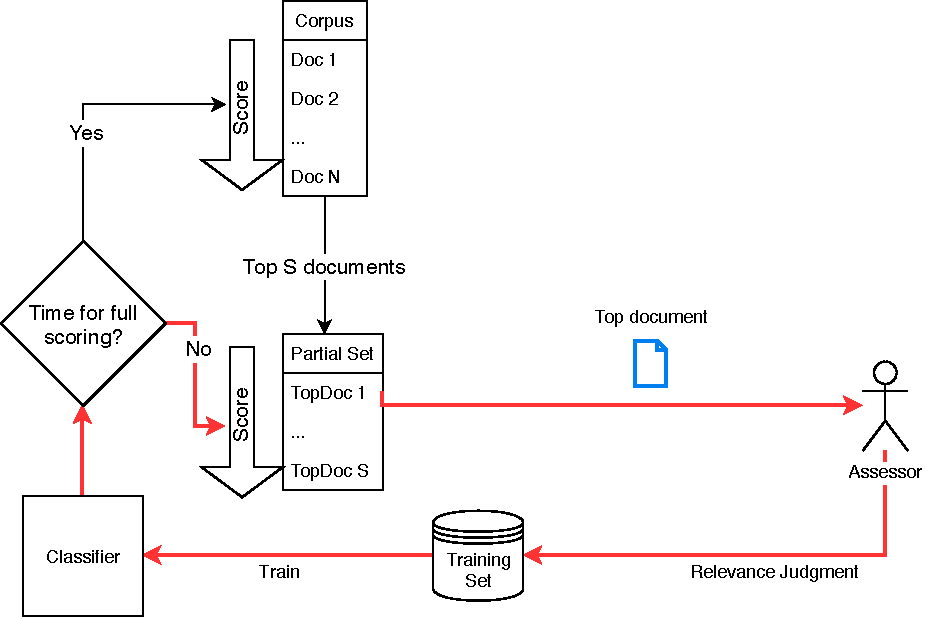
\includegraphics[width=1.0\textwidth]{animation/partial1.pdf}
 \caption{After every judgment}
\end{figure}
\end{frame}

\begin{frame}{Partial Refresh Strategy}
\begin{figure}
 \centering 
 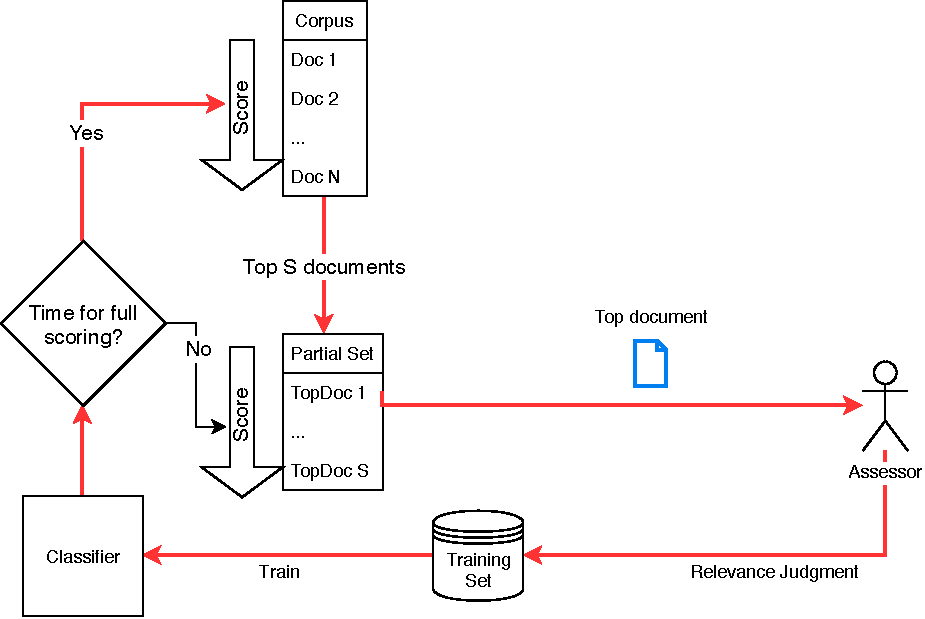
\includegraphics[width=1.0\textwidth]{animation/partial2.pdf}
 \caption{After every K judgments}
\end{figure}
\end{frame}

\begin{frame}{Precision Based Refreshing}
Refresh when ``output quality'' falls below some threshold

\pause
\vskip 1cm
\textbf{Problem:} Defining ``output quality''

\pause
\vskip 1cm
Refresh when the precision of the last $m$ assessed documents fall below $p$
\end{frame}

\begin{frame}{Precision Based Refreshing}
\begin{figure}
 \centering 
 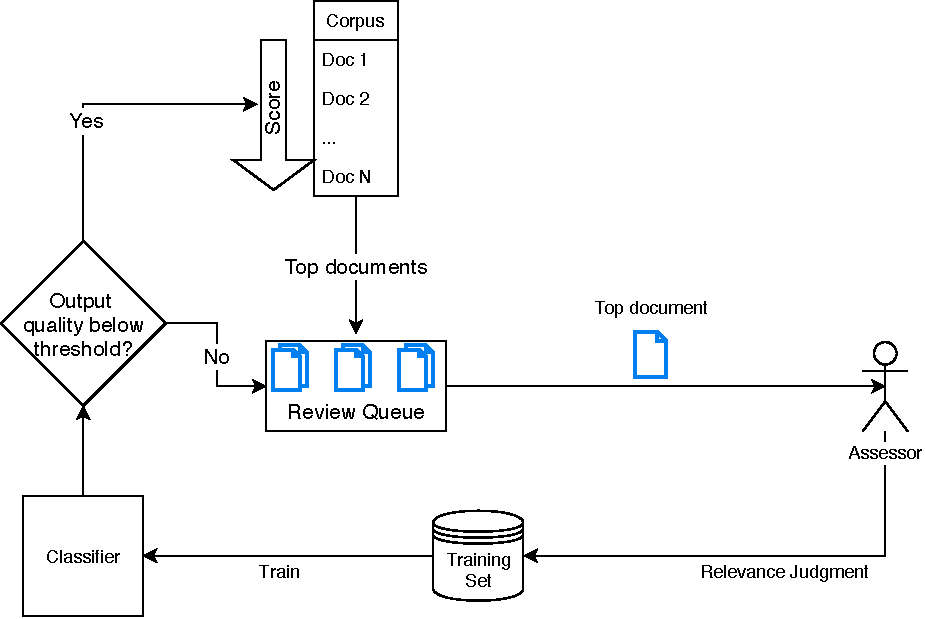
\includegraphics[width=1.0\textwidth]{animation/prec.pdf}
\end{figure}
\end{frame}

\begin{frame}{Dataset and Experiment}
    \begin{itemize}
        \item \texttt{Athome1} test collection from the TREC 2015 Total Recall track
        \item Around 290k documents; 10 topics
        \item Implementation of CAL from
            HiCAL\footnote{\url{http://hical.github.io}}
        \item Recall at certain effort
            \begin{itemize}
                \item Normalized Effort = No. of Assessments / Total no. of
                    relevant documents
            \end{itemize}
        \item Simulation running time
    \end{itemize}
\end{frame}

\begin{frame}{Results}
\begin{table}[]
\centering
\caption{BMI vs Static Batch Refreshing}
\label{table.summary}
\resizebox{\textwidth}{!}{%
\begin{tabular}{|c|c|c|c|c|c|}
\hline
\textbf{Strategy} & \begin{tabular}[x]{@{}c@{}}
    \textbf{Avg. Recall}\\ \textbf{@($E_{norm}$=1)}
\end{tabular} & \begin{tabular}[x]{@{}c@{}}
\textbf{Avg. Recall}\\ \textbf{@($E_{norm}$=2)}
\end{tabular} & \begin{tabular}[x]{@{}c@{}}
\textbf{$E_{norm}$ for}\\ \textbf{75\% recall}
\end{tabular}&
\begin{tabular}[x]{@{}c@{}}
    \textbf{Running Time}\\ \textbf{(in min)}
\end{tabular} \\ \hline \hline
\texttt{bmi}& 0.715 & 0.905 & 1.128 & 0.22 \\ \hline \hline
\rowcolor{LightCyan}
\texttt{static(k=1)} & 0.750 & 0.926 & 1.021 & 49.29 \\ \hline
\texttt{static(k=100)} &  0.704 & 0.887 & 1.167 & 0.47 \\ \hline
\end{tabular}
}
\end{table}
\vskip 0.5cm
\texttt{bmi}: exponentially increasing batch size
\texttt{static(k)}: fixed batch size of \texttt{k}
\end{frame}

\begin{frame}{Results}
\begin{table}[]
\centering
\caption{Partial Refresh Strategy}
\label{table.summary}
\resizebox{\textwidth}{!}{%
\begin{tabular}{|c|c|c|c|c|c|}
\hline
\textbf{Strategy} & \begin{tabular}[x]{@{}c@{}}
    \textbf{Avg. Recall}\\ \textbf{@($E_{norm}$=1)}
\end{tabular} & \begin{tabular}[x]{@{}c@{}}
\textbf{Avg. Recall}\\ \textbf{@($E_{norm}$=2)}
\end{tabular} & \begin{tabular}[x]{@{}c@{}}
\textbf{$E_{norm}$ for}\\ \textbf{75\% recall}
\end{tabular}&
\begin{tabular}[x]{@{}c@{}}
    \textbf{Running Time}\\ \textbf{(in min)}
\end{tabular} \\ \hline \hline
\rowcolor{LightCyan}
\texttt{static(k=1)} & 0.750 & 0.926 & 1.021 & 49.29 \\ \hline \hline
\texttt{partial(k=10,s=1000)} &  0.753 & 0.926 & 1.008 & 40.92 \\ \hline
\rowcolor{LightCyan}
% \texttt{partial(k=100,s=500)} &  0.753 & 0.923 & 1.022 & 38.28 \\ \hline
% \rowcolor{LightCyan}
\texttt{partial(k=100,s=1000)} &  0.754 & 0.922 & 1.013 & 39.57 \\ \hline
\rowcolor{LightCyan}
\texttt{partial(k=100,s=5000)} &  0.756 & 0.921 & 1.016 & 40.70 \\ \hline
\texttt{partial(k=500,s=1000)} &  0.700 & 0.815 & 1.324 & 38.63\\
\hline
\end{tabular}
}
\end{table}
\vskip 0.5cm
\texttt{static(k)}: fixed batch size of \texttt{k}

\texttt{partial(k,s)}: complete scoring after \texttt{k} judgments, partial set
size of \texttt{s} documents
\end{frame}

\begin{frame}{Results}
\begin{table}[]
\centering
\caption{Partial Refresh Strategy}
\label{table.summary}
\resizebox{\textwidth}{!}{%
\begin{tabular}{|c|c|c|c|c|c|}
\hline
\textbf{Strategy} & \begin{tabular}[x]{@{}c@{}}
    \textbf{Avg. Recall}\\ \textbf{@($E_{norm}$=1)}
\end{tabular} & \begin{tabular}[x]{@{}c@{}}
\textbf{Avg. Recall}\\ \textbf{@($E_{norm}$=2)}
\end{tabular} & \begin{tabular}[x]{@{}c@{}}
\textbf{$E_{norm}$ for}\\ \textbf{75\% recall}
\end{tabular}&
\begin{tabular}[x]{@{}c@{}}
    \textbf{Scoring Time}\\ \textbf{(in min)}
\end{tabular} \\ \hline \hline
\rowcolor{LightCyan}
\texttt{static(k=1)} & 0.750 & 0.926 & 1.021 & 23.88 \\ \hline \hline
\texttt{partial(k=10,s=1000)} &  0.753 & 0.926 & 1.008 & 2.25 \\ \hline
% \rowcolor{LightCyan}
% \texttt{partial(k=100,s=500)} &  0.753 & 0.923 & 1.022 & 38.28 \\ \hline
\rowcolor{LightCyan}
\texttt{partial(k=100,s=1000)} &  0.754 & 0.922 & 1.013 & 0.39 \\ \hline
\rowcolor{LightCyan}
\texttt{partial(k=100,s=5000)} &  0.756 & 0.921 & 1.016 & 0.82 \\ \hline
\texttt{partial(k=500,s=1000)} &  0.700 & 0.815 & 1.324 & 0.17 \\
\hline
\end{tabular}
}
\end{table}
\vskip 0.5cm
\texttt{static(k)}: fixed batch size of \texttt{k}

\texttt{partial(k,s)}: complete scoring after \texttt{k} judgments, partial set
size of \texttt{s} documents
\end{frame}

\begin{frame}{Results}
\begin{table}[]
\centering
\caption{Precision Based Refreshing}
\label{table.summary}
\resizebox{\textwidth}{!}{%
\begin{tabular}{|c|c|c|c|c|c|}
\hline
\textbf{Strategy} & \begin{tabular}[x]{@{}c@{}}
    \textbf{Avg. Recall}\\ \textbf{@($E_{norm}$=1)}
\end{tabular} & \begin{tabular}[x]{@{}c@{}}
\textbf{Avg. Recall}\\ \textbf{@($E_{norm}$=2)}
\end{tabular} & \begin{tabular}[x]{@{}c@{}}
\textbf{$E_{norm}$ for}\\ \textbf{75\% recall}
\end{tabular}&
\begin{tabular}[x]{@{}c@{}}
    \textbf{Running Time}\\ \textbf{(in min)}
\end{tabular} \\ \hline \hline
\rowcolor{LightCyan}
\texttt{static(k=1)} & 0.750 & 0.926 & 1.021 & 49.29 \\ \hline \hline
\texttt{precision(m=25,p=0.4)} &  0.698 & 0.915 & 1.129 & 35.68 \\ \hline
\texttt{precision(m=25,p=0.6)} &  0.735 & 0.923 & 1.059 & 40.20 \\ \hline
\rowcolor{LightCyan}
\texttt{precision(m=25,p=0.8)} &  0.750 & 0.926 & 1.024 & 44.64 \\ \hline
\rowcolor{LightCyan}
\texttt{precision(m=25,p=1.0)} &  0.752 & 0.926 & 1.014 & 47.41 \\
\hline
\end{tabular}
}
\end{table}
\vskip 0.5cm
\texttt{static(k)}: fixed batch size of \texttt{k}

\texttt{precision(m,p)}: perform refresh when precision of last \texttt{m}
documents fall below \texttt{p}
\end{frame}


% \begin{frame}{Recency Weighting}
% Recent judgments ``weighted'' more in training
% \vskip 1cm

% \textbf{Default training:} loss computed based on a random positive and a negative judgment (numerous iterations)

% \pause
% \vskip 0.5cm
% \textbf{Modified training:} latest judgment is $w$ times more likely to be
% sampled than the first judgment (fit a linear curve).
% \end{frame}


% \begin{frame}{Recency Weighting}
% With original settings, recency weighting didn't result in any difference

% \vskip 1cm
% \textbf{Possible Reason:} Very high number of training iterations ($it = 10^5$)
% \end{frame}


% \section{Outline}



% \section{Implementation}
% \begin{frame}{Implementation}
% \begin{itemize}
%     \item Implementation of BMI in C++
%     \begin{itemize}
%         \item Fast
%         \item Easy to use and configure (CLI/HTTP)
%         \item Extendable (components as abstractions  which can be replaced/modified easily)
%     \end{itemize}
%     \item Useful research tool
%     \item Used in
%     \begin{itemize}
%         \item TREC 2017 Core Track effort by UWatMDS
%         \item User Study and Demo (papers submitted to SIGIR 2018)
%     \end{itemize}
%     \item Operates entirely in-memory
%     \begin{itemize}
%         \item Requires all the documents in the memory (Drawback)
%     \end{itemize}
% \end{itemize}
% \end{frame}


% \subsection{Static Batch Sizes}
% \begin{frame}{Static Batch Sizes}
% Train and score all documents after every $k$ assessments ($k$ is static)
% \vskip 1cm
% $k = 1$
% \begin{itemize}
% \item Effective
% \item High computation cost
% \end{itemize}
% \end{frame}


% \begin{frame}
% \begin{figure}
%  \centering 
%  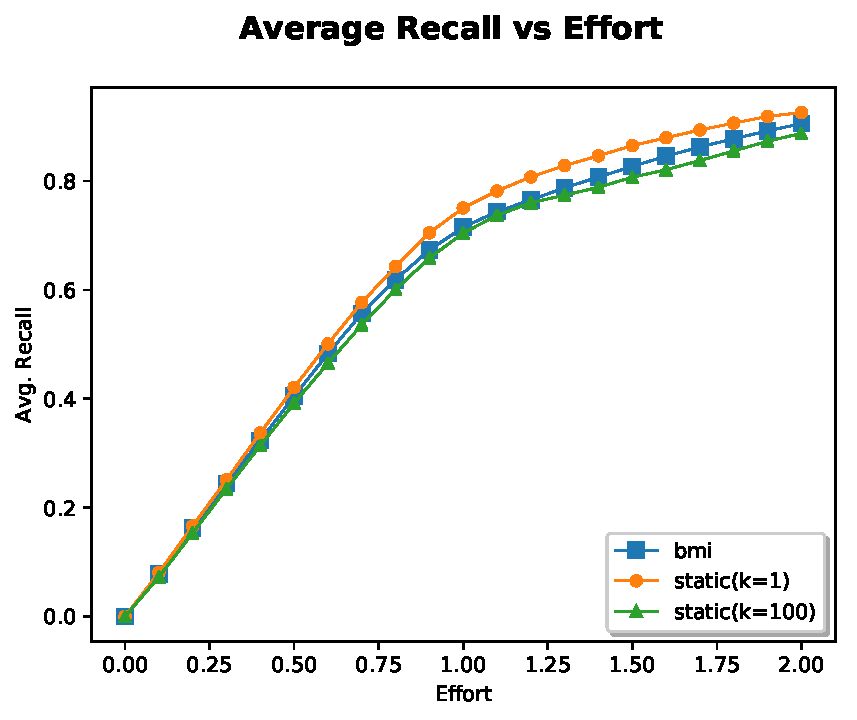
\includegraphics[width=1.0\textwidth]{static1.pdf}
% \end{figure}
% \end{frame}



% \begin{frame}{Partial Refresh}
% This strategy can help with the high memory costs
% \vskip 0.5cm
% Partial Refreshes are fast and performed on small set of data which can be stored in the memory

% \vskip 0.25cm
% Full Refresh can be performed in the background (reading from disk)
% \end{frame}


% \begin{frame}
% \begin{figure}
%  \centering 
%  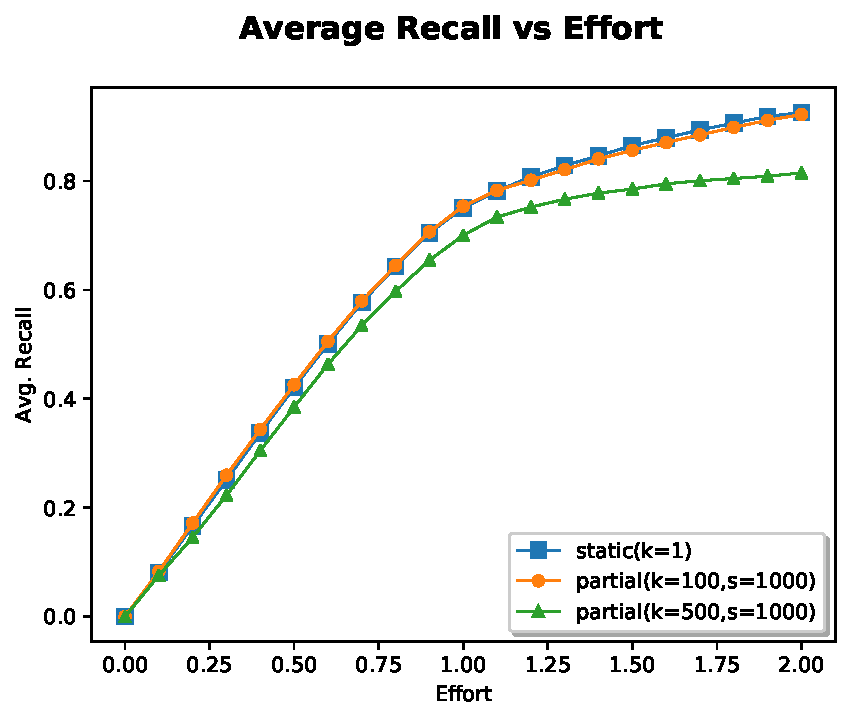
\includegraphics[width=1.0\textwidth]{partial1.pdf}
% \end{figure}
% Parameters
% \begin{itemize}
%     \item Size of partial re-score document set ($s$)
%     \item Period for full refresh ($k$)
% \end{itemize}
% \end{frame}


% \begin{frame}
% \begin{figure}
%  \centering 
%  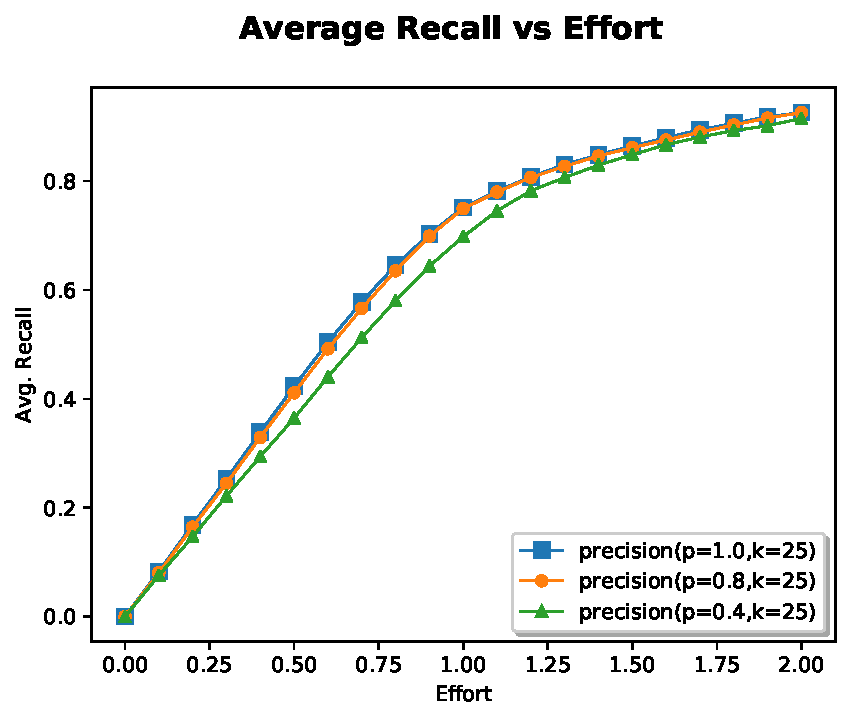
\includegraphics[width=1.0\textwidth]{prec1.pdf}
% \end{figure}
% \end{frame}

% \begin{frame}
% \begin{figure}
%  \centering 
%  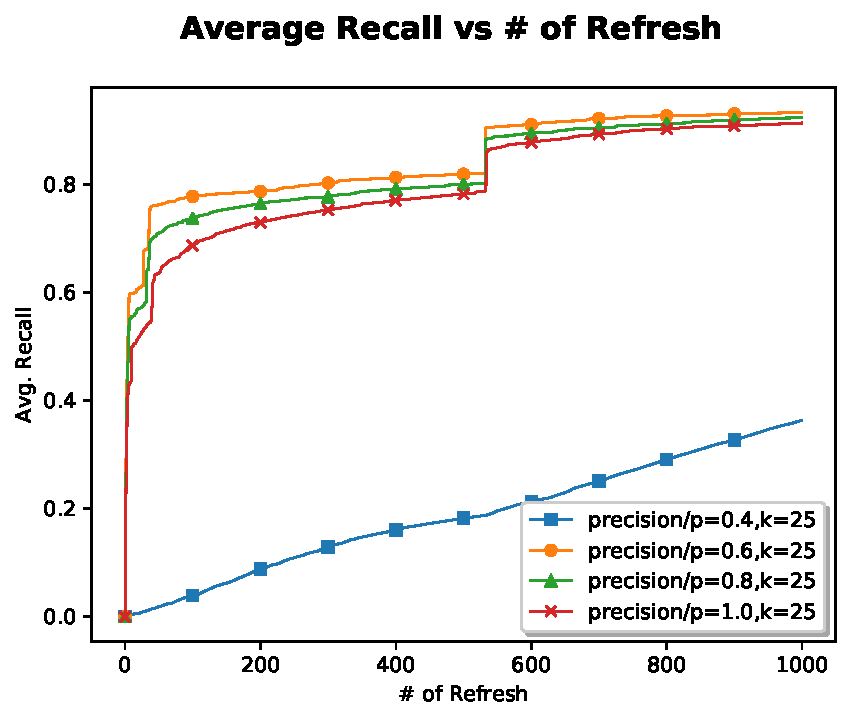
\includegraphics[width=1.0\textwidth]{prec2.pdf}
% \end{figure}
% \end{frame}


% \begin{frame}
% \begin{figure}
%  \centering 
%  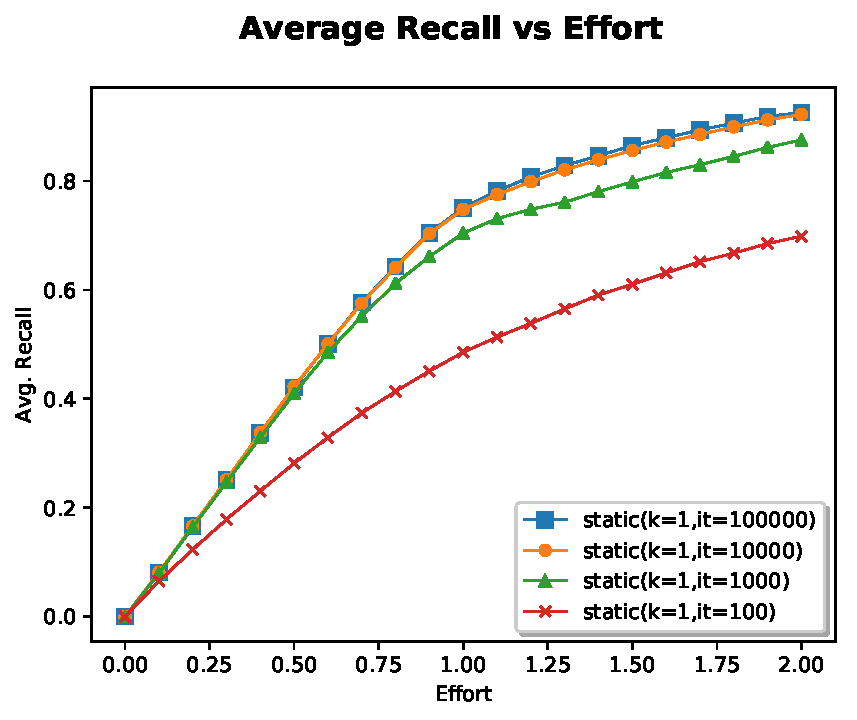
\includegraphics[width=1.0\textwidth]{train1.pdf}
% \end{figure}
% \end{frame}

% \begin{frame}
% \begin{figure}
%  \centering 
%  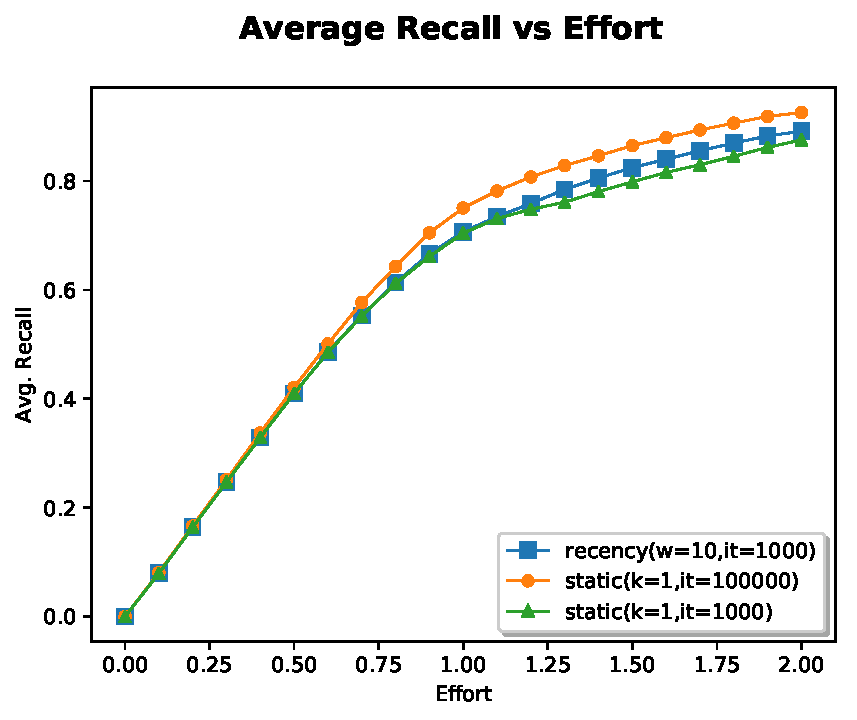
\includegraphics[width=1.0\textwidth]{rec1.pdf}
% \end{figure}
% \end{frame}

\section{Conclusion}
\begin{frame}{Summary}
\begin{itemize}
    \item Frequent refreshing helps achieving higher recall using lesser
       assessment effort
       \vskip 0.5cm
    \item Static batch size of 1 performs great but is computationally expensive
        \begin{itemize}
            \item Practical for reasonably sized datasets and modern hardware 
            \item Various alternative strategies can achieve similar
                effectiveness with reduced computations
        \end{itemize}
\end{itemize}
\pause
\centering
\textbf{Questions?}
\end{frame}

\end{document}

